\chapter{Introduction}     % numéroté
\section{Bref historique}
%
\lettrine[nindent=0em,lines=2]{L}{}a découverte des rayons X par Wilhelm Roentgen en 1895, suivie de la radioactivité par Henri Becquerel en 1896, ainsi que le radium par Pierre et Marie Curies en 1898 ont été des événements qui ont révolutionné le monde médical sur le plan diagnostic (naissance de la radiologie), et thérapeutique (naissance de la radiothérapie). Ces découvertes ont ouvert la voie aux traitements de nombreuses maladies réfractaires aux traitements connus à l’époque.  Cependant, la radiothérapie a souffert pendant longtemps des possibilités limitées de la technologie et de la physique. Les traitements étaient par exemple essentiellement limités aux cancers superficiels (peau), certaines tumeurs ORL \nomenclature{ORL}{Oto-Rhino-Laryngologie} et aux traitements palliatifs et antalgiques; les générateurs à l’époque ne pouvant produire que le rayonnement X ayant un faible pouvoir pénétrant (100-400 kV). Le développement des générateurs de Van de Graaff et des bêtatrons en fin des années 1930 et début des années 1940 a rendu possible l’accélération des électrons aux énergies de quelques MeV pour le Van de Graaff et environ 10 MeV pour les bêtatrons, ce qui a favorisé l’essor de la radiothérapie externe avec les faisceaux du mégavoltage. Le bêtatron est devenu l’accélérateur de choix après la seconde guerre mondiale et, durant la même période, le développement des accélérateurs linéaires médicaux a vu le jour en utilisant les sources de micro-ondes utilisées dans les systèmes radars, mais le bêtatron restait la technologie la plus utilisée pour les applications médicales à cause de sa faible complexité et son faible coût. Les progrès sur le développement des accélérateurs linéaires ont progressivement supplanté l’utilisation des bêtatrons pour les applications médicales, au profit des accélérateurs linéaires médicaux que l’on retrouve dans tous les départements de radio-oncologie de par le monde. L’autre alternative à l'époque, et sur laquelle repose notre projet était la curiethérapie, qui par opposition à la radiothérapie externe, est une forme de radiothérapie qui consiste à placer les sources radioactives scellées, soit directement dans le volume tumoral ou soit à proximité de celui-ci. Elle fait partie des principales modalités de traitement des tumeurs cancéreuses, notamment : la radiothérapie (externe, curiethérapie), la chimiothérapie et la chirurgie. La curiethérapie permet de délivrer une dose élevée localement dans le volume tumoral, tout en épargnant les tissus sains périphériques. Le début de la curiethérapie s’est fait avec la poudre de radium encapsulée dans des tubes ou aiguilles de platine. Les tubes de radium étaient insérés dans les cavités utérines et vaginales pour traiter les cancers du col, et les aiguilles étaient implantées dans le volume tumoral pour le traitement de certaines tumeurs telles que, le cancer de la peau ou de la langue. Par la suite, les aiguilles de radium ont été progressivement remplacées par les fils d'Iridium-192, améliorant ainsi l’efficacité et la tolérance au traitement. Les avancées technologiques et la meilleure connaissance des propriétés physiques des sources radioactives, ainsi que les effets radiobiologiques des rayonnements ionisants se sont avérées être les piliers de la pratique de la curiethérapie moderne de ce $21^{\grave{e}me}$ siècle.
%
\section{Différents types de curiethérapie}
Étant donné que les différentes formes de curiethérapie peuvent se différentier en fonction du type d’implant et de sa durée, de l’intensité de la source radioactive et du type de chargement de celle-ci, on envisager la classification de la curiethérapie en fonction de chacun de ces facteurs. Les tableaux \ref{TypeImplant}, \ref{DureeImplant} et  \ref{TypeChargement} résument ce classement respectivement en fonction du type d’implant, sa durée et le type de chargement de la source. La classification par débit de dose telle que défini par l’ICRU  \cite{ICRU} est :
%
\begin{itemize}[label=\textbullet, font=\LARGE]
\item \textbf{Bas débit de dose : 0.4-2 Gy/h}\newline
Forme de curiethérapie utilisée pour le traitement la cavité buccale, la prostate, les sarcomes et le cancer de l’oropharynx.
%
\item \textbf{Débit de dose moyen} : 2-12 Gy/h\newline
La littérature indique que ce débit de dose, également connu sous le nom de \enquote{débit de dose intermédiaire} est rarement utilisé en pratique puisqu’il conduirait à une exposition excessive si un tel implant était chargé manuellement. D’autre part, dans quelques cas où cette gamme de débit de dose a été utilisée, les résultats cliniques se sont avérés pauvres par rapport à ceux que l’on obtient pour la technique bas débit de dose ou haut débit de dose \cite{Podgorsak}.
%
\item \textbf{Haut débit de dose} : > 12 Gy/h \newline
Forme de curiethérapie indiquée pour le traitement du cancer des poumons, de l’œsophage, des seins, du col de l’utérus et de la prostate.
\end{itemize}
%
Il existe également la curiethérapie par débit de dose pulsé (1-3 Gy/h) qui est une nouvelle technique apparue dans les années 1990. Cette technique simule les traitements faits à bas débit de dose en délivrant de petites fractions de dose, sous forme d’impulsion de durée entre 10-15 min. La source d’Iridium-192 est utilisée avec une intensité 10 à 20 fois plus faible que dans le cas des applications à haut débit de dose. Ces fractions de dose sont délivrées une fois toutes les heures et nécessitent une hospitalisation du patient.\newline
La curiethérapie peut être administrée en monothérapie pour les petites tumeurs de la peau (paupières, nez, oreilles, lèvres, cavité orale), ou pour le traitement du cancer de la prostate précoce à faible risque. Elle peut également être pratiquée en complément à la radiothérapie externe (boost). Les traitements en boost concernent les tumeurs de grande taille pour lesquelles les limites sont difficiles à définir avec une bonne précision. Enfin, la curiethérapie peut succéder une chirurgie.
%
\begin {table}[http]
%\begin {center}
\caption{Classification en fonction du type d’implant.}
\label{TypeImplant} 
\renewcommand{\arraystretch}{1.4}
	\begin{tabular}{p{5.5cm} p{9.0cm}}
		\toprule[1.25pt]
        \hline
        Type d'implant         &                            Description   \\ 
        \hline
		Intracavitaire         & Sources placées dans une cavité naturelle au contact direct de la tumeur (vagin, utérus, 				nasopharynx). \\ 
		Interstitielle 	   	   & Sources placées à l’intérieur du volume tumoral (peau, lèvre, sein, langue, anus, prostate). \\ 
		Surface (moule)        & Sources placées à la surface du tissu à traiter (œil, mélanome). \\ 
		Intraluminale          & Sources placées dans une cavité de petit diamètre (œsophage, bronche, canal biliaire). \\ 
        Intraoperative         & Sources implantées dans le volume tumoral par chirurgie. \\ 
        Intravasculaire        & Sources placées dans de petites ou grandes artères. \\
        \bottomrule[1.25pt]
	\end{tabular} 
	%\end {center}
\end {table}
%
\begin {table}[ht!]
%\begin {center}
\caption{Classification en fonction de la durée de l’implant.}
\label{DureeImplant} 
\renewcommand{\arraystretch}{1.4}
	\begin{tabular}{p{5.5cm} p{9.0cm}}
		\toprule[1.3pt]
        \hline
        Type d'implant     &                            Description   \\ 
        \hline
        Permanent          &  La dose est délivrée jusqu’à la décroissance radioactive complète de la source. \\ 
		Temporaire  	   & L’irradiation est délivrée sur une courte période de temps et les sources sont retirées dès que la dose prescrite est atteinte. \\ 
        \bottomrule[1.3pt]
	\end{tabular} 
	%\end {center}
\end {table}
%
\begin {table}[ht!]
\caption{Classification en fonction du type de chargement.}
\label{TypeChargement} 
\renewcommand{\arraystretch}{1.4}
	\begin{tabular}{p{5.5cm} p{9.0cm}}
		\toprule[1.3pt]
        \hline
        Type de chargement       &                            Description   \\ 
        \hline
        Chargement à chaud       & Les sources radioactives sont d’abord chargées dans l’applicateur et celui-ci est ensuite inséré  		 dans le patient.\\ 
		Chargement différé 	     &  Les applicateurs sont d'abord implantés dans le volume à irradier et les sources radioactives 		  sont ensuite chargées, soit manuellement (chargement différé manuel) ou automatiquement par un projecteur de source. \\ 
        \bottomrule[1.3pt]
	\end{tabular} 
\end {table}
%
Plus d’une douzaine d’isotopes radioactifs ont historiquement été utilisés pour les traitements en curiethérapie, mais les sources les plus utilisées sont : ${}^{60}$Co, ${}^{137}$Cs, ${}^{192}$Ir, ${}^{125}$I, ${}^{103}$Pd et ${}^{90}$Sr/${}^{90}$Y, toutes émetteur de photons. L’utilisation du ${}^{226}$Ra et du ${}^{222}$Rn a été progressivement abandonnée, principalement à cause des problèmes de radioprotection qu’elles posent. Ces sources sont commercialisées sous forme d’aiguilles, de grains, de fils souples, d’épingles ou de capsules cylindriques. Le tableau \ref{Sources} ci-dessous résume leurs caractéristiques physiques\cite{Podgorsak, Baltas@2006}. La curiethérapie haut débit de dose (HDD) \nomenclature{HDD}{Haut Débit de Dose} à l’Hôtel-Dieu de Québec (HDQ) \nomenclature{HDQ}{Hôtel-Dieu de Québec} est réalisée avec un projecteur de source de type Flexitron, commercialisé par la compagnie Elekta, et contenant une source d'${}^{192}$Ir dont le schéma est présenté à la figure \ref{Flexitron} \cite{Alizadeh}.
%
\vspace{2.0cm}
\begin {table}[!ht]
\caption{Caractéristiques physiques de certains isotopes  utilisés en curiethérapie. La demie-vie est exprimée en années (a) ou en jours (j). HVL (Half-Value Layer) est la couche de demi-atténuation. \nomenclature{HVL}{Half-Value Layer}}
\label{Sources} 
\renewcommand{\arraystretch}{1.4}
	\begin{tabular}{p{1.8cm} p{1.9cm} p{1.9cm} p{1.9cm}p{2.5cm} p{2.8cm}}
	\toprule[1.25pt]
       \hline
        Isotope & $\stackrel{-}{E_{\gamma}}$ (MeV) & Demie-vie  &  HVL (Pb) (mm)  &  Activité (GBq.mg$^{-1}$) & Type d'implant \\ 
         \hline
        Co-60      &      1,25     &    5,26 a    &    11     &     41.91    &   Temporaire  \\ 
        Cs-137     &      0,66     &     30 a     &    6,5    &     3,202    &   Temporaire  \\ 
        Au-198     &      0,41     &    2.7 j     &    2,5    &     9055,12  &   Permanent    \\ 
        Ir-192     &      0,38     &    73,8 j    &     3     &     340.98   &   Temporaire   \\ 
        I-125      &      0,028    &    60 j      &    0,02   &     650,15   &   Permanent ou temporaire \\ 
        Pa-103     &      0,021    &    17 j      &    0,01   &     2763,13  &   Permanent   \\ 
        \bottomrule[1.25pt]
	\end{tabular} 
\end{table}
%
\begin{figure}[!ht]
\centering
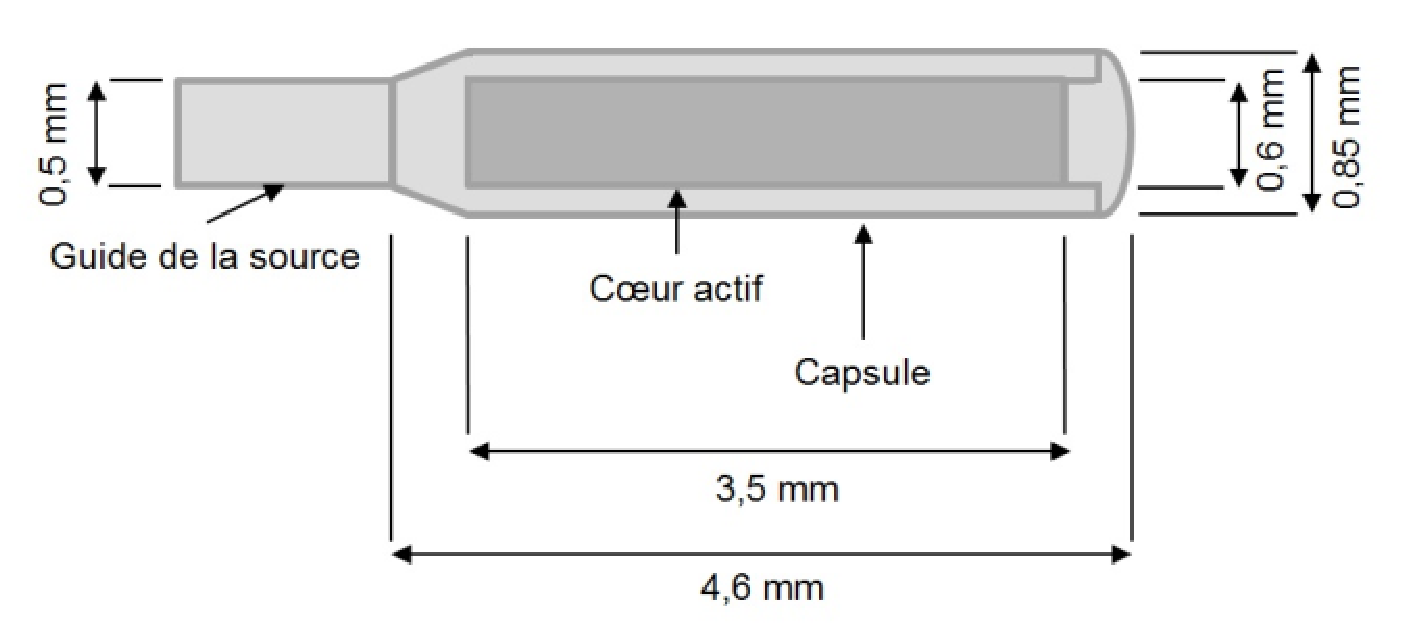
\includegraphics[width=11.0cm,height=5.0cm]{Flexitron.eps}
\caption{\label{Flexitron} Schéma de la composition de la source d’Iridium-192 se trouvant dans le Flexitron de la compagnie Elekta (Alizadeh et al., 2015).}
\end{figure}
%
\section{Équipement de traiment}
La forme de la curiethérapie sur laquelle repose le présent projet est la curiethérapie haut débit de dose (HDD) pour le cancer de la prostate. Les équipements nécessaires pour délivrer ce type de traitement sont un gabarit qui guide l’implantation des cathéters dans la prostate (figure \ref{GabaritProstate}). Le geste du radio-oncologue dans l’implantation des cathéters est guidé par une échographie transrectale (figure \ref{ImagerieSonde}). Lorsque tous les cathéters sont implantés, le patient passé au scanner pour l’acquisition des images pour la dosimétrie et par la suite, un projecteur de source contenant une source d’Iridium-192 est utilisé pour la délivrance de la dose (figure \ref{ProjecteurSource}).
%
\begin{figure}[http]
\centering
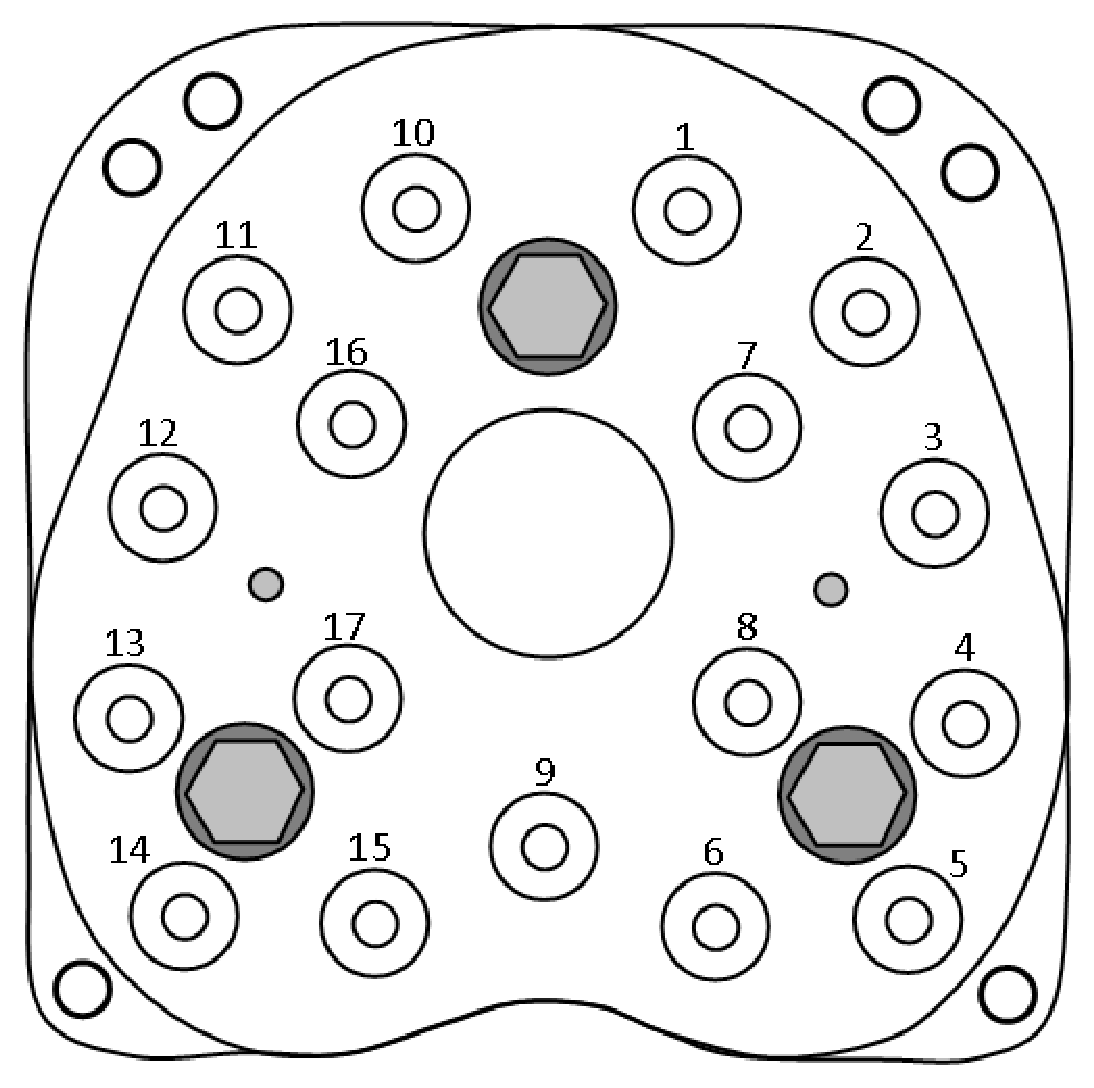
\includegraphics[width=5.5cm,height=5.3cm]{GabaritProstate.eps}
\caption{\label{GabaritProstate} Gabarit de Nucletron utilisé en curiethérapie de la prostate pour l’implantation des cathéters.}
\end{figure}
%
Les différents équipements cités ci-dessus appartiennent à une chaîne globale de traitement en curiethérapie HDD, qui s’étend de la phase diagnostique jusqu’à la délivrance de la dose. Lors de l’acquisition de ces équipements, leurs normes de fonctionnement qui avaient été considérées comme étant acceptables par le biais d’une phase de commissionnement, doivent être maintenues tout le long de leur durée d’exploitation, d’où l’intérêt d’un programme de contrôle qualité (CQ). \nomenclature{QC}{Contrôle Qualité} Ce programme de CQ s’insère dans d’un cadre plus global d’un programme d’assurance qualité de l’Hôpital. La section qui suit décrit les grandes lignes d’un programme de CQ en curiethérapie HDD et la phase de ce programme dans laquelle s’inscrit ce projet.
%
\begin{figure}[!ht]
\centering
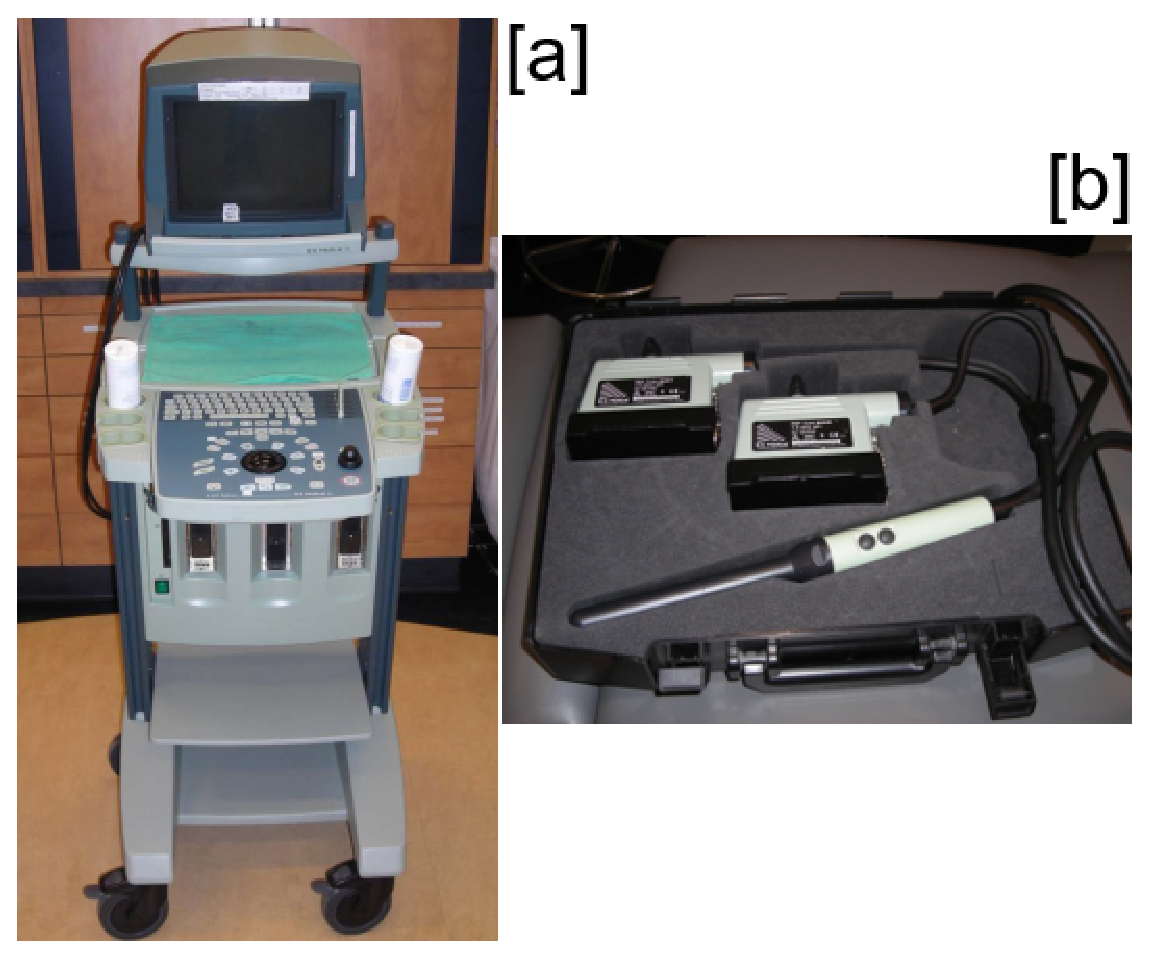
\includegraphics[width=8.5cm,height=6.5cm]{ImagerieSonde.eps}
\caption{\label{ImagerieSonde} Système d’échographie pour la localisation de la prostate et le guidage d’implantation des cathéters. Console d’acquisition et de visualisation (a) et sonde transrectale (b).}
\end{figure}
%
\begin{figure}[!ht]
\centering
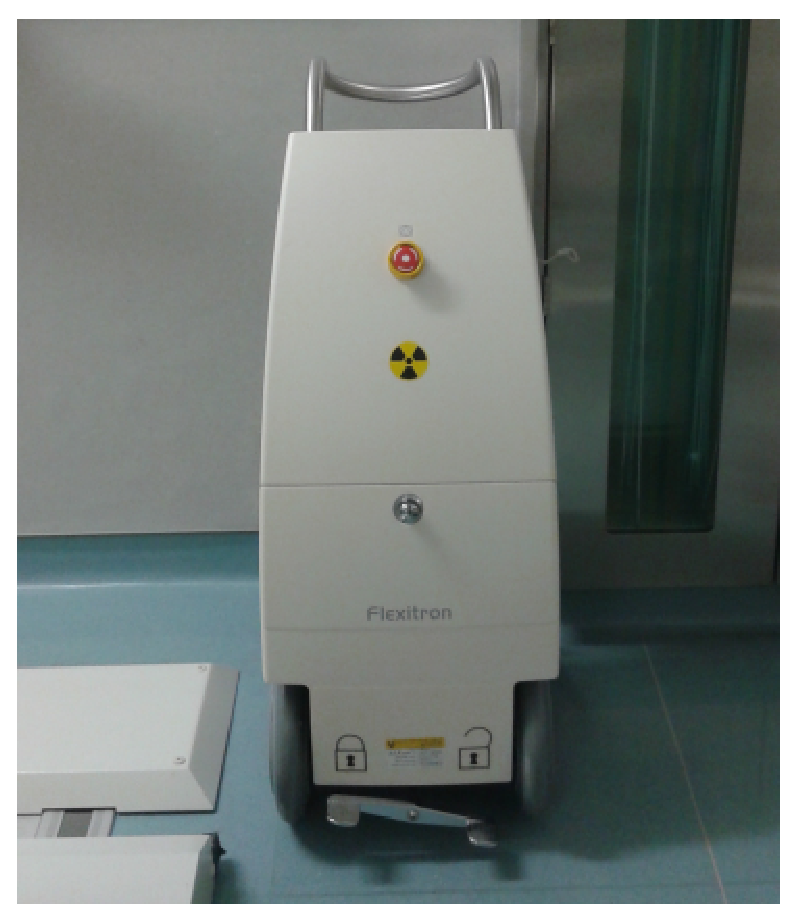
\includegraphics[width=6.0cm,height=7.0cm]{ProjecteurSource.eps}
\caption{\label{ProjecteurSource} Projecteur de source de marque Flexitron de la compagnie Elekta contenant une source d’Iridium-192.}
\end{figure}
%
\vspace{3cm}
\section{Assurance qualité et contrôle qualité en curiethérapie HDD}
\subsection{Assurance qualité}
L’assurance qualité (AQ) \nomenclature{AQ}{Assurance Qualité} et le CQ sont deux aspects importants en radiothérapie qui permettent de garantir la fiabilité et la précision de la dose délivrée au patient. Un programme d’AQ bien établi réduit les incertitudes et les erreurs dans la dosimétrie, la planification du traitement, la performance des équipements, la délivrance de la dose et, par conséquent, garantit la réalisation des objectifs cliniques.
%
\begin{itemize}[label=\textbullet, font=\LARGE]
	\item \textbf{Définition générale}\newline
	L'assurance qualité est l'ensemble des actions planifiées et systématiques nécessaires pour assurer avec une confiance 			suffisante qu'un produit ou un service satisfait aux exigences de qualité \cite{Podgorsak}.
    %
	\item \textbf{AQ en radiothérapie} \newline
	Dans le contexte de la radiothérapie, l’AQ est l’ensemble des procédures qui garantissent la cohérence d’une prescription 		médicale et l’exécution sécuritaire de celle-ci afin de délivrer la dose prescrite au volume cible, tout en minimisant la dose 		aux tissus normaux alentour, l’exposition du personnel et en garantissant la surveillance convenable du patient en vue 			d’évaluer le résultat final du traitement. Une telle définition englobe plusieurs aspects sur le plan organisationnel 			concernant, notamment, la prise en charge et le suivi adéquat des patients, la répartition des responsabilités, la formation et 	la gestion des équipements \cite{Podgorsak, Lisbona}.
\end{itemize}
% 
\subsection{Contrôle qualité}
Le  CQ est un des éléments essentiels d’un programme d’AQ si l’on veut garantir un niveau de confiance élevé dans l’utilisation des équipements, ou des procédés qui interviennent dans la chaîne de traitement. Il s’agit donc d’un processus réglementaire par lequel les performances réelles de la qualité sont mesurées par rapport aux normes existantes, et les mesures nécessaires sont prises pour maintenir, ajuster, ou corriger ces performances si les écarts de conformité aux normes sont observés.\newline 
En curiethérapie HDD, le contrôle qualité concerne:
%
\begin{itemize}[label=\textbullet, font=\LARGE]
\item Les équipements d'imagerie qui sont à la base du diagnostic, et qui fournissent des informations utiles pour la planification du trainement, à savoir, Le scanner, l’imagerie par résonance magnétique (IRM), \nomenclature{IRM}{Imagerie par Résonance Magnétique} la tomographie d’émission monophotonique couplée au scanner (SPECT/CT), \nomenclature{SPECT}{Single-Photon Emission Computed Tomography} la tomographie par émission de positons couplée au scanner (PET/CT) \nomenclature{PET}{Positron Emission Tomography} et l’échographie (CT). \nomenclature{CT}{Computed Tomography (Scanner)}
%
\item Les projecteurs de sources qui permettent de délivrer la dose au patient en assurant la radioprotection de ce dernier et celle du personnel.
%
\item les systèmes de planification de traitement (TPS) et les algorithmes de calcul de dose qui leur sont associés.
\end{itemize}
%
Le présent projet dont un des aspects est l’introduction d’un nouveau concept du CQ, s’insère dans la phase de la planification du traitement en curiethérapie HDD pour le cancer de la prostate.
%
\section{Le cancer de la prostate}     % numéroté
\subsection{Incidence et mortalité}
Le cancer est classé par l’Organisation Mondiale de la Santé (OMS) \cite{OMS} \nomenclature{OMS}{Organisation Mondiale de la Santé} comme étant la deuxième cause de mortalité dans le monde. Les dernières statistiques de GLOBOCAN 2012 \cite{GLOBOCAN} publiées en décembre 2013 estiment à 14,1 millions, le nombre de nouveaux cas de cancer et à 8,2 millions le nombre de décès liés au cancer survenus en 2012, en comparaison respectivement à 12,7 et 7,6 millions en 2008. L’OMS souligne qu’en 2015, 8,8 millions de décès sont attribués au cancer et que, près d’un décès sur 6 dans le monde est dû au cancer. Ces chiffres interpelant peuvent s’expliquer par plusieurs facteurs, entre autres : la croissance démographique et le vieillissement de la population, une augmentation de la prévalence des facteurs de risques bien établis tels que le tabagisme, le surpoids et l’inactivité physique \cite{Torre}. Sur le plan national, la publication \enquote{statistique canadienne sur le cancer} diffusée le 20 juin 2017 \cite{StatCanada} indique que le cancer est la première cause de mortalité au Canada, soit \textasciitilde 30\% par rapport aux autres maladies. La figure \ref{FigureStatCancer1} \cite{StatCanada} illustre le taux de mortalité au Canada en 2012, pour l’ensemble des causes de décès confondus.
%
\begin{figure}[ht]
\centering
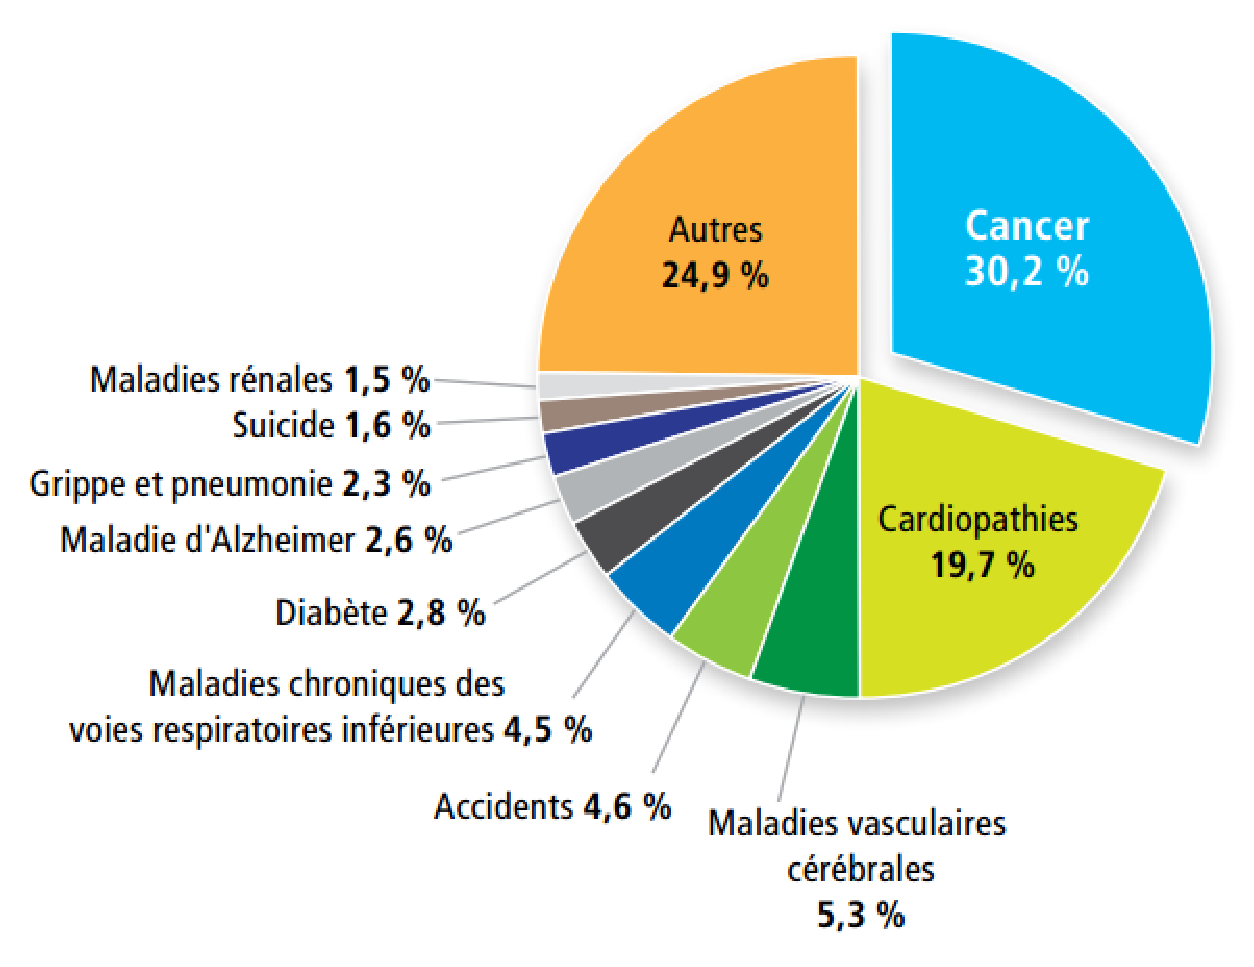
\includegraphics[width=7.3cm,height=5.5cm]{FigureStatCancer1.eps}
\caption{\label{FigureStatCancer1} Taux de mortalité au Canada en 2012, toutes causes confondues.}
\end{figure}
%
Les estimations sur l’incidence (respectivement pour la mortalité) pour les hommes en 2017 sont \textasciitilde 100 000 (respectivement 42 600) nouveaux cas. La projection de nouveaux cas en 2017 pour le cancer de la prostate est 20,7\%, suivi du cancer colorectal (14.5\%) et le cancer des poumons et bronches (14\%). Les chiffres sans doute alarmants présentés ci-dessus, aussi bien sur le plan mondial que national, peuvent expliquer la grande mobilisation observée dans le monde pour la recherche sur le cancer; recherches orientées soit dans le perfectionnement des méthodes de traitements actuellement utilisées en clinique, ou dans le développement de nouvelles possibilités thérapeutiques.
%
\subsection{Anatomie et physiologie}
La prostate fait partie du système génital masculin. Chez les jeunes hommes, elle a la taille d’une noix qui augmente progressivement de volume à la fin de la quarante et début de la cinquante. Elle joue un rôle important pour la fertilité de l’homme, notamment, en participant à la formation et la maturation des spermatozoïdes. Sa localisation lui confère également un rôle dans le bon fonctionnement de l’appareil mictionnel étant donné qu’elle est étroitement liée aux deux sphincters qui assurent une bonne continence urinaire. Comme le montre la figure \ref{FigureProstate} \cite{ImageProstate}, la position de la glande prostatique est dans le petit bassin. Sur sa partie supérieure appelée base, repose la partie inférieure de la vessie. Elle est localisée en arrière du pubis et devant le rectum. Les organes à risques primordiaux qui compromettent la dosimétrie pour le cancer de la prostate sont la vessie, le rectum et l’urètre dont une partie est contenue dans la prostate (urètre prostatique).
%
\begin{figure}[ht]
\centering
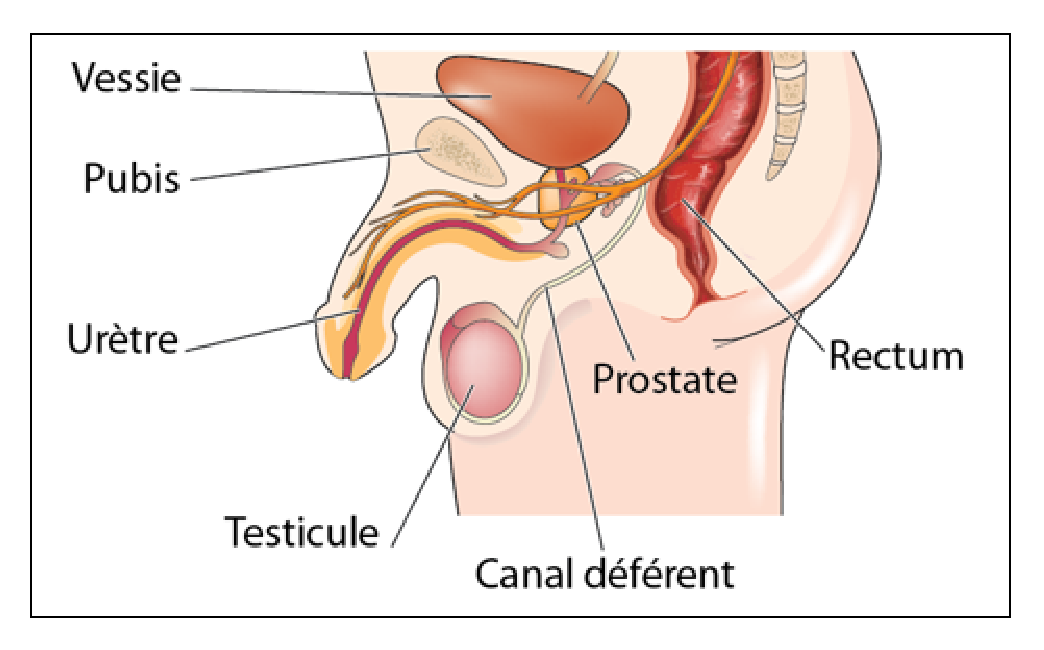
\includegraphics[width=8.5cm,height=6.5cm]{FigureProstate.eps}
\caption{\label{FigureProstate} Anatomie de la prostate et sa localisation par rapport à la vessie et le rectum.}
\end{figure}
%
\subsection{Diagnostique}
L’approche standard pour le diagnostic du cancer de la prostate repose sur la combinaison des résultats d’un test d’antigène prostatique spécifique (APS) \nomenclature{APS}{Antigène Prostatique Spécifique}, le toucher rectal (TR) \nomenclature{TR}{Toucher Rectal} permettant de vérifier la taille et la forme de la prostate, une échographie transrectale (ETR) \nomenclature{ETR}{Échographie Transrectale} ou une biopsie. Il existe une certaine complémentarité entre les différents examens cités ci-dessus; par exemple, le médecin peut faire recours à une ETR pour le diagnostic du cancer de la prostate si l’APS est élevé ou si une région anormale a été détectée lors du TR.   La connaissance du stade du cancer est un élément clé dans cette phase de dépistage, puisque celle-ci détermine le choix de la modalité de traitement, ainsi que le pronostic sur la survie du patient. Cette stadification clinique est effectuée par les médecins en s’appuyant sur le système international TNM \cite{Sobin} dans lequel, \enquote{T} désigne le type de la tumeur, \enquote{N} la présence de la tumeur dans les ganglions lymphatiques et \enquote{M} la présence de la tumeur dans d’autres régions éloignées (métastases). Le tableau \ref{StadificationProsatate} ci-dessous résume cette stadification clinique pour les différents types de tumeurs et les détails de la classification N et M relatifs à leur caractère envahissant peuvent être consultés dans les travaux de Sobin et al.\cite{Sobin}. La stadification TNM est toujours associée au score de Gleason \cite{Chen, Salomon} créé dans les années 1960-1970 et redéfini en 2005, score qui fait référence au degré d’agressivité du cancer de la prostate.
%
\begin {table}[ht]
%\begin {center}
\caption{Stadification clinique du cancer de la prostate en fonction du type de la tumeur.}
\label{StadificationProsatate} 
\renewcommand{\arraystretch}{1.4}
	\begin{tabular}{p{5.5cm} p{9.0cm}}
		\toprule[1.3pt]
        \hline
        Stadification clinique                   &      Description   \\ 
        \hline
        T1               			   & Ce stade concerne les tumeurs de petites tailles se limitant à la prostate, invisibles à l'imagerie et pour lesquelles, il est impossible de palper par le biais du toucher rectal. Il s’agit d’un stade qui ne produit généralement aucun symptôme.                                  \\ 
        T2               			   & La tumeur est détectable par le toucher rectal, mais limitée à la prostate.                               \\ 
        T3               			   & Ce stade concerne les tumeurs pour lesquelles les cellules cancéreuses se sont propagées au-delà de la prostate, mais localisables dans les régions qui entourent la glande.                                \\
        T4               			   & Tumeurs pour lesquelles les cellules cancéreuses se sont propagées au-delà de la prostate dans les structures avoisinantes (sphincter externe, rectum, muscles releveurs de l’anus ou paroi pelvienne).                                \\ 
        M               			   & Il s’agit d’un stade pour lequel la tumeur s’est propagée dans les régions éloignées (métastase), au-delà de la prostate (os, foie, poumons) par l’intermédiaire du système lymphatique et/ou par la circulation sanguine.                                 \\ 
        \bottomrule[1.3pt]
	\end{tabular} 
	%\end {center}
\end {table}
%
\subsection{Place de l'imagerie pour la curiethérapie de la prostate HDD}
Ces dix dernières années ont été marquées par des avancées technologiques qui ont rendu possible l’utilisation de l’imagerie prostatique dans le processus de détection, localisation et stadification du cancer de la prostate, en complément de l’APS, le TR, l’ETR ou la biopsie. Les principales modalités d’imagerie telles que le scanner, l’échographie, l’IRM et le PET sont actuellement utilisées pour la localisation des cellules cancéreuses et la détermination de leur extension dans les structures éloignées de la prostate (métastases), la stadification, le guidage en temps réel de l’implantation des cathéters dans la glande, ainsi que la surveillance active du patient. Les paragraphes suivants sont consacrés à la description succincte de quelques-unes de ses techniques, ainsi que leurs principales utilisations.
%
\subsection*{\textbf{Échographie prostatique}}
L’échographie est la technique d’imagerie la plus ancienne et reste largement parmi les techniques les plus utilisées dans le processus de prise en charge du cancer de la prostate. Les indications de cette technique sont, entre autres, le guidage en temps réel du prélèvement des échantillons de tissus prostatiques pour la biopsie et l’implantation des cathéters dans la prostate, une délinéation claire de la prostate ainsi que la détermination de son volume \cite{Sarkar, Taneja, Dubinsky, Kirkham, Holm2002}. Le principe physique de la technique repose sur la mesure des ondes mécaniques de compression se propageant dans un milieu tissulaire. La propagation de ces ondes à l’interface de deux tissus ayant des propriétés acoustiques différentes obéit aux lois analogues à celles de l’optique ondulatoire (réflexion, réfraction, diffusion et absorption). Le signal qui résulte de la partie réfléchie de l’onde est recueilli par un transducteur (émetteur et récepteur d’impulsions ultrasonores), traité et synthétisé en ton de gris des tissus pour produire une image statique ou dynamique. L’impédance acoustique qui est une caractéristique propre à chaque tissu, et responsable de l’imagerie échographique est donnée par l’équation \eqref{eqn:imp} dans laquelle, $\rho \left(kg/m^{3}\right)$ est la densité des tissus et $c \left(m/s\right)$ la vitesse du son  qui varie en fonction du type de tissu dans lequel la propagation a lieu.
%
\begin{equation}\label{eqn:imp}
	z = \rho \times c
\end{equation}
%
Les différences de densité et de vitesse de propagation à l’interface des tissus sont donc des propriétés fondamentales pour la génération des échos et le contraste dans le processus de formation de l’image échographique. Cependant, les systèmes médicaux approximent généralement la vitesse des ondes dans les milieux biologiques à celle des tissus mous, soit 1540 m/s \cite{Bushberg}, seule la densité est donc prise en compte pour la différenciation des différents tissus. Les coefficients de transmission (T) et réflexion (R) d’une onde acoustique arrivant normalement à l’interface de deux tissus d’impédances acoustiques z$_{1}$ et z$_{2}$ sont donnés par l’équation \eqref{eqn:reflex_Trans},
%
\begin{equation}\label{eqn:reflex_Trans}
	T = \frac{4z_{1}z_{2}}{\left(z_{1}+z_{2}\right)^{2}}, \qquad R = 1-T
\end{equation}
%
L’équation \eqref{eqn:reflex_Trans} explique la nécessité de l’utilisation d’un gel entre le transducteur et la peau, aux interfaces muscle-air; la transmission étant \textasciitilde 100\% en l’absence du gel \cite{ EPoulin}. L’inconvénient majeur de l’échographie est son contraste tissulaire limité entre le tissu cancéreux et bénin, limitation qui est grandement améliorée par l’imagerie par résonance magnétique.
%
\subsection*{\textbf{Imagerie par résonance magnétique}}
L’imagerie par résonance magnétique (IRM) présente un avantage de produire des images anatomiques avec une résolution en contraste relativement élevée, ce qui permet un meilleur diagnostic du cancer de la prostate. L’IRM anatomique (pondération T$_{2}$) est généralement associée à l’IMR fonctionnelle (séquences de perfusion et de diffusion) pour les examens cliniques de routine \cite{Horwitz}. Une telle combinaison qui est connue sous le nom de l’IMR multiparamétrique, conduit à des résultats plus fiables que les images pondérées T$_{2}$ seulement pour le diagnostic initial, le bilan d’extension métastatique, la présence de grade de Gleason élevé et la surveillance active du patient. Le principe physique de l’IRM repose sur les propriétés magnétiques de la matière. En effet, le corps humain est constitué en grande partie (environ 70\%-80\% du poids du corps) par les molécules d’eau (H$_{2}$O). Les noyaux d’atomes d’hydrogène sont constitués d’un proton qui, du point de vue magnétique, sont assimilables à des petits moments magnétiques de spin ($\mu$). En l’absence d’un champ magnétique externe, l’orientation de ces moments magnétiques est aléatoire dans la matière, ce qui conduit à une aimantation macroscopique (M) nulle. L’application d’un champ magnétique externe B$_{0}$ fait tourner les moments magnétiques de spin autour de la direction de B$_{0}$ et chaque moment décrit un cône de révolution autour de cette direction, ce qui fait apparaître une aimantation longitudinale M$_{z}$ et transversale M$_{xy}$. En présence de du champ B$_{0}$, le processus d’acquisition de l’image passe d’abord par une phase d’excitation par une onde radiofréquence (RF) à la fréquence dite de Larmor ($\nu_{0}$, fréquence de résonance du système) donnée par l’équation \eqref{eqn:FLarmor1} dans laquelle $\gamma$ représente le rapport gyromagnétique.
%
\begin{equation}\label{eqn:FLarmor1}
	\nu_{0}= \frac{\gamma}{2\pi}B_{0}
\end{equation}
%
Cette excitation va créer une situation de déséquilibre dans laquelle, l’aimantation longitudinale va décroitre et la composante transversale va croitre. L’intensité et la durée de l’impulsion RF déterminent l’angle de basculement. À la fin de l’impulsion RF, l’aimantation revient à sa position d’équilibre (phénomène de relaxation) tout en émettant un signal (courant induit dû à la décroissance exponentielle de M$_{xy}$) qui est recueilli par des antennes réceptrices. Le retour à l’équilibre se fait pendant un intervalle de temps T$_{2}$ pour l’aimantation transversale et T$_{1}$ pour l’aimantation longitudinale. T$_{2}$ est caractéristique de chaque tissu, ce qui permet de différentier les différents tissus excités. Cependant, le signal recueilli provient de tout l’échantillon, d’où la nécessité d’une technique de codage par application d’un gradient de champ magnétique dans la même direction que B$_{0}$ (gradient de sélection de coupe G$_{z}$) donnée par la relation :
%
\begin{equation}\label{eqn:Gradient}
	B(z)= B_{0}+G_{z}z
\end{equation}
%
La fréquence de résonance du système prend donc la forme de l’équation \eqref{eqn:FLarmor2}, ce qui permet de sélectionner le volume anatomique à explorer et d’analyser que le signal provenant de ce dernier.
%
\begin{equation}\label{eqn:FLarmor2}
	\nu_{z}= \frac{\gamma}{2\pi}B(z)
\end{equation}
%
La position de chaque point dans le volume anatomique excitée est par la suite encodée par application d’un grandirent de codage en phase et en fréquence dans l’espace de fourrier. Ce codage spatial en fréquence et en phase permet par la suite, moyennant une transformation de Fourier du signal, de reconstruire l’image de la coupe. Les détails complémentaires sur le principe physique de l’IRM peuvent être consultés dans la littérature \cite{Bushberg, Grover, HENDEE}. Les deux inconvénients majeurs de l’IRM sont la nature statique des images reconstruites et le coût d’acquisition de la technologie élevée.
%
\subsection*{\textbf{Scanner abdomino-pelvien}}
Les images CT continuent à avoir leur place dans le processus de prise en charge du cancer de la prostate. Dans la phase diagnostique, ils permettent la recherche de métastases ganglionnaires chez les patients à risque élevé ou intermédiaire. Ces images sont également déterminantes lors de la phase de planification, notamment pour la reconstruction des cathéters et le calcul prévisionnel de la dose. Le principe physique de cette technique repose sur l’atténuation des photons émis par un tube à rayons X. En effet, lors de la traversée d’un faisceau de rayons X dans un milieu d’épaisseur $x$, les photons subissent plusieurs types d’interactions physiques avec les atomes du milieu, conduisant à leur absorption ou leur diffusion. Si l’on désigne par I$_{0}$ l’intensité du faisceau à l’entrée du milieu, l’intensité de ce dernier à la sortie après un parcours d’épaisseur $x (cm)$ est régit par une loi d’atténuation exponentielle donnée par l’équation \eqref{eqn:APhotons},
%
\begin{equation}\label{eqn:APhotons}
	I(x)= I_{0} exp\left(-\mu x\right)
\end{equation}
%
$\mu (cm^{-1})$ est le coefficient d’atténuation linéaire qui dépend du numéro atomique du milieu, sa densité et l’énergie du rayonnement incident. Techniquement, le scanner est une chaîne radiologique constituée d'un tube à rayons X et un ensemble de détecteurs disposés en couronne. Au cours de l’acquisition, l’ensemble tube-détecteurs tourne autour du patient pendant que la table avance en continu à vitesse constante (acquisition hélicoïdale), ou avance après l’acquisition des données d’une coupe (acquisition séquentielle). Les détecteurs transforment l’énergie radiante des photons X en signal électrique dont l’amplitude est proportionnelle à l’intensité du faisceau incident. Un profil d’atténuation regroupe la totalité des signaux électriques générés par tous les détecteurs pour un angle de rotation donné. Plusieurs profils d’atténuation à différents angles de rotation sont enregistrés, échantillonnés et numérisés. Ces données sont ensuite rétro-projetées dans une matrice de reconstruction, puis transformées en image.  En effet, la matrice de données est composée de n lignes et  n colonnes, chaque élément de cette matrice est un pixel contenant une valeur d’atténuation ou de densité dans l’échelle des gris. Les coefficients d’atténuation des différents tissus sont normalisés à celui de l’eau et exprimés en unités Hounsfield (UH), en l’honneur de Sir Godfrey Hounsfield qui a été l’un des principaux innovateurs de la technologie CT, selon l’équation \eqref{eqn:Hounsfield},
%
\begin{equation}\label{eqn:Hounsfield}
	UH\left(x, y, z\right)= 1000 \left[\frac{\mu\left(x,y,z\right)-\mu_{eau}}{\mu_{eau}}\right]
\end{equation}
% 
$\mu\left(x,y,z\right)$ est la valeur moyenne du coefficient d’atténuation linéaire pour un élément de volume (voxel) du tissu dans le patient, à la position $(x, y, z)$ et $\mu_{eau}$ le coefficient d'atténuation linéaire de l'eau pour le spectre des rayons X utilisé. Une telle normalisation conduit à UH$_{eau}=0$, -1000 (air), 280 à 230 (tissus adipeux).
%
\section{Planification du traitement en radiothérapie}
De façon générale, les TPS sont utilisés en radiothérapie pour générer la balistique du traitement permettant d’obtenir une distribution de dose prescrite et uniforme dans le volume cible, tout en minimisant l’irradiation des tissus sains alentour \cite{Thomadsen1, Venselaar, Gerbaule}. La prise en charge d’un patient pour un traitement en radiothérapie est subdivisée en plusieurs étapes, la première étant la phase du diagnostic (acquisition d’images diagnostiques, stadification de la tumeur, bilan d’extension, score de Gleason, etc.). Cette première phase va conduire à la décision de traiter et au choix de la modalité de traitement si le diagnostic est positif. La deuxième phase consiste en l’acquisition des images permettant le contourage du volume cible et les OARs environnants à l’aide des modalités d’imagerie telles: le CT, l’IRM, l’échographie, etc. Le processus de contourage du volume cible devant recevoir la dose prescrite est guidé par les recommandations de la commission internationale des unités et mesures radiologiques (ICRU) dans ces rapports 50 et 62 \nomenclature{ICRU}{International Commission on Radiation Units and Measurements} \cite{ICRU50, ICRU62}. Ces recommandations définissent un vocabulaire cohérent sur la définition des volumes cibles, reconnu et compris au niveau de chaque institution, et au niveau international. Les principaux volumes définis dans ces recommandations sont :
%
\begin{itemize}[label=\textbullet, font=\LARGE]
\item \textbf{Volume tumoral macroscopique (GTV)} : \nomenclature{GTV}{Gross Tumour Volume} \newline
Il est constitué par l’ensemble des lésions tumorales, mesurables, palpables ou visibles avec une des modalités d’imagerie actuelle. 
%
\item \textbf{Volume cible anatomoclinique (CTV)}: \nomenclature{CTV}{Clinical Target Volume}\newline
Il comprend le volume anatomique dans lequel on veut éradiquer la maladie (GTV) et les extensions microscopiques des cellules cancéreuses qui peuvent être considérées avec une certaine probabilité comme pertinentes pour le traitement. Il s’agit d’une expansion géométrique autour du GTV pour tenir compte des incertitudes anatomocliniques.
%
\item \textbf{Volume cible prévisionnel (PTV)}: \nomenclature{PTV}{Planning Target Volume }\newline
Il s’agit d’un concept géométrique introduit pour les besoins de la planification et de l’évaluation. Il est défini pour assurer avec une probabilité cliniquement acceptable que la dose prescrite est délivrée dans le CTV. Ce volume vise à tenir compte des variations de la position du CTV, de sa forme et de ses dimensions; variations dues aux mouvements du patient ou de ses organes (respiration, battements cardiaques, remplissage de la vessie ou du rectum, déglutition). Il tient également compte des incertitudes liées à l'imperfection de la balistique du traitement.
%
\end{itemize}
%
Cette phase de courage des volumes d’intérêt est suivie du calcul prévisionnel de la distribution de dose qui sera délivrée au patient avec un TPS. Il s’agit de la phase durant laquelle toute la balistique du traitement est mise en place.\newline
Dans le cas particulier de la planification du cancer de la prostate en curiethérapie HDD, l’ordre des étapes décrites ci-dessus est quelque peu modifié. Après la phase diagnostique conduisant à la décision de traiter en curiethérapie HDD, le radio-oncologue procède à la mise en place des cathéters dans la glande prostatique à l’aide d’un gabarit sous guidage échographique. L'implantation des cathéters se fait au bloc opératoire, sous anesthésie générale. Par la suite, une série d’images est prise au CT, ces images visent deux objectifs principaux :
%
\begin{itemize}[label=\textbullet, font=\LARGE]
	\item Permettre le contourage de toutes structures anatomiques d'intérêt, notamment, la prostate, l'urètre, la vessie et le 	rectum.
    %
	\item Permettre la reconstruction des cathéters. En effet, les cathéters sont distinguables des tissus biologiques, car ils 	sont faits d’un matériau CT compatible pour la réduction des artéfacts métalliques et ils contiennent de l’air.
    %
\end{itemize}
%
Contrairement à la radiothérapie externe, la planification avec le TPS en curiethérapie HDD consistera à déterminer les positions de la source radioactive dans chaque cathéter (dwell positions) et le temps d’arrêt de la source à chacune des positions (dwell time). En planification inverse, les objectifs cliniques du traitement, c’est-à-dire, la couverture du CTV et la limitation de la dose aux OARs sont introduits dans le TPS et servent de point de départ pour trouver le plan optimal (meilleure combinaison dwell position et dwell time). Il s’agit d’un processus itératif au cours duquel, l’algorithme de calcul implanté dans le TPS explore l'espace des solutions (plans de traitement réalisables) et le planificateur adopte le plan qui satisfait le mieux les objectifs cliniques. Les sections \ref{sssec:TG-43} et \ref{sssec:optimis} qui suivent sont consacrées à la présentation du formalisme TG-43 et une brève description de quelques algorithmes d’optimisation implantés dans les TPS.
%
\subsection{Formalisme du calcul de dose: AAPM TG-43}\label{sssec:TG-43} 
\nomenclature{AAPM}{American Association of Physicists in Medicine}
En 1995, le groupe de travail N$^{o} 43$ \cite{AAPMTG-43} de l'American Association of Physicists in Medicine (AAPM) a publié un rapport sur la dosimétrie des sources utilisées en curiethérapie interstitielle. Ce rapport, suivi de ces mises à jour publiées en 2004 et 2017 \cite{AAPMTG-43R1, AAPMTG-43R2} présentent le formalisme de calcul de dose utilisé dans tous les TPS actuels. Il convient cependant de souligner que le formalisme TG-43 a été initialement développé pour la dosimétrie des sources en curiethérapie bas débit de dose telles que l'${}^{125}$I et le ${}^{103}$Pd, mais ce dernier est largement accepté sur le plan international et utilisé pour la dosimétrie des sources à haute énergie pour la curiethérapie HDD et débit de dose pulsé \cite{Venselaar}. Ces recommandations introduisent de nouvelles quantités physiques telles que : le débit de kerma de référence ($S_{k}$), la constante de débit de dose ($\Lambda$), la fonction de dose radiale ($g(r)$), la fonction d’anisotropie ($F(r, \theta)$) et la fonction géométrique ($G(r, \theta)$). Le formalisme permet de calculer la distribution de dose en tous points d’un plan passant par l’axe longitudinal de la source, le milieu étant considéré comme infini, homogène et constitué d’eau. La figure \ref{FigureTG-43} montre le système de coordonnées utilisé pour le calcul de la dose en tout point $P(r, \theta)$.
%
\begin{figure}%[h]
\centering
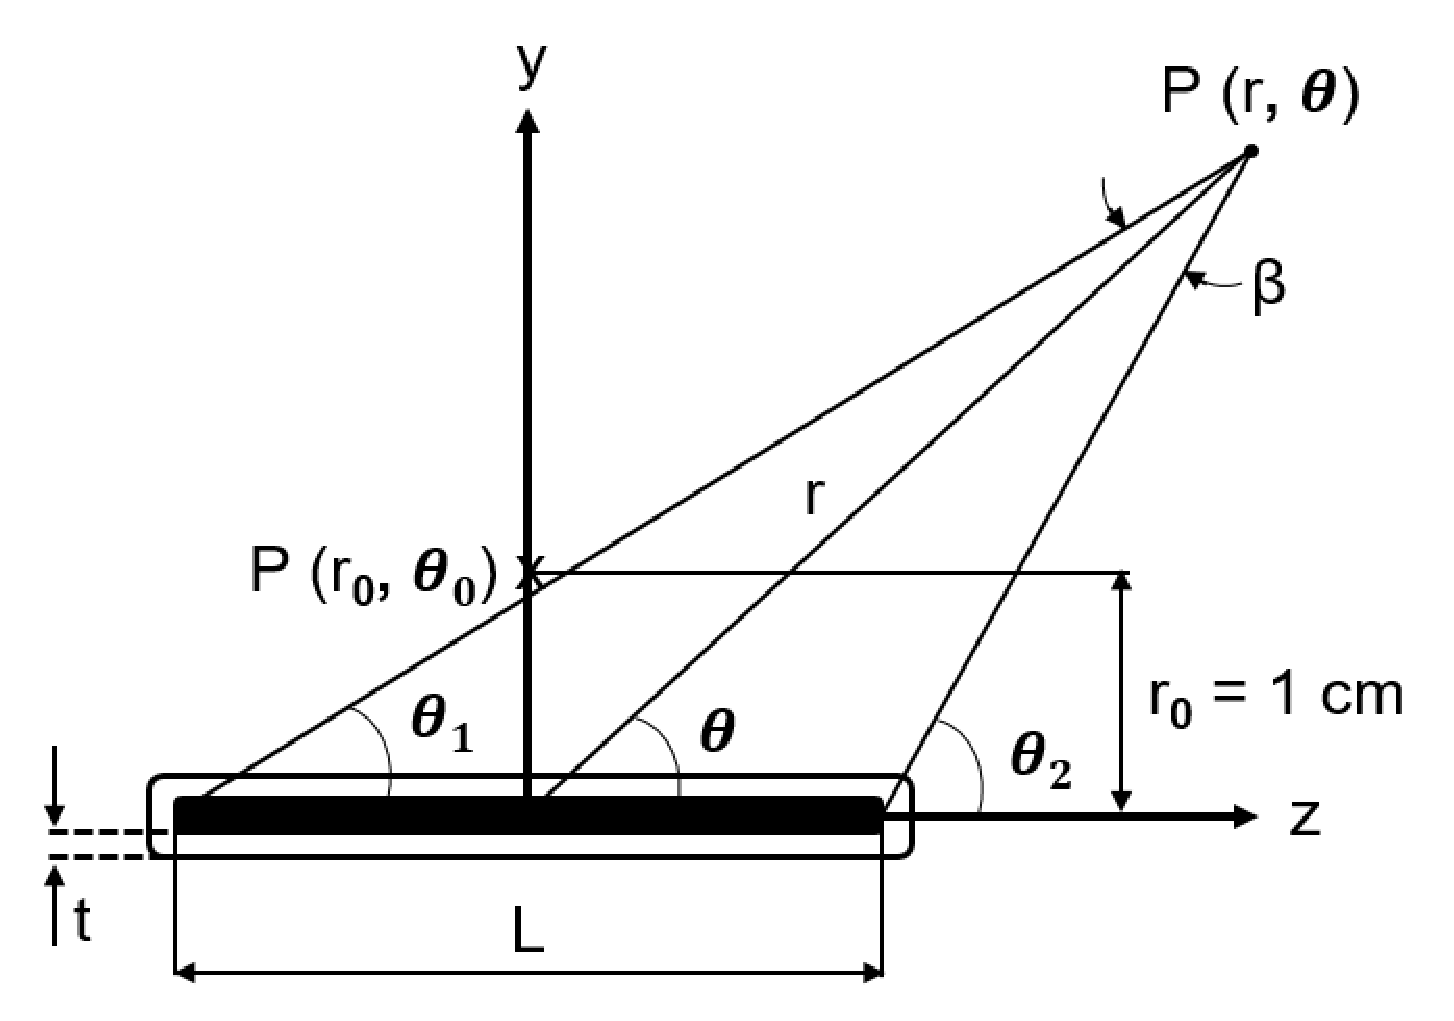
\includegraphics[width=8.0cm, height=6.0cm]{FigureTG-43.eps}
\caption{\label{FigureTG-43} Système de cordonnées utilisé pour le calcul de dose dans le formalisme TG-43 (Nath et al., 1995).}
\end{figure}
%
Le débit de dose $\stackrel{.}{D} (r, \theta)$ dans l’approximation d’une source linéaire est donné par l’équation générale,
%
\begin{equation}\label{eqn:DoseRef}
	\stackrel{.}{D}\left(r,\theta\right)=S_{k}.\Lambda . \frac{G_{L}\left(r,\theta\right)}{G_{L}\left(r_{0},\theta_{0}\right)}.g_{L}\left(r\right).F\left(r,\theta\right)
\end{equation}
%
dans laquelle les différents paramètres signifient :
%
\renewcommand{\arraystretch}{1.5}
\begin{longtable}{p{1.5cm} p{13.4cm}}
r & La distance du centre de partie active de la source au point de calcul $P(r, \theta)$. \\
%
$r_{0}$ & La distance de référence, 1 cm dans le plan transverse de la source à l’angle $\theta = 90^{0}$.\\
%
$S_{k}$ & Le débit de kerma de référence dans l’air exprimé en $\mu Gym^{2} h^{-1}$ et généralement mesuré à 1 m du centre de la source dans le plan transverse de celle-ci. Il représente la puissance de la source. \\
%
$\Lambda$ & La constante de débit de dose : $\Lambda (cGy h^{-1} U^{-1})$ avec $U=\mu Gym^{2} h^{-1}$   permet la conversion du débit de kerma dans l'air au débit de dose dans l'eau au point de référence $P(r_{0}, \theta_{0})$.\\
%
$G_{L}(r, \theta)$ & La fonction géométrique : elle permet d’améliorer la précision des calculs due à l’interpolation des valeurs à partir des données tabulées de la constante de débit de dose à des points discrets. Du point de vue physique, cette fonction apporte une correction de l’effet de la loi de l’inverse carré de la distance, au détriment des phénomènes d’atténuation et de diffusion. \\
%
$g_{L}(r)$ & La fonction de dose radiale, elle prend en compte la diminution du débit de dose sur l’axe traverse de la source due uniquement aux phénomènes de diffusion et d’absorption. \\
%
$F(r, \theta)$ & La fonction d’anisotropie : la variation angulaire des phénomènes d'absorption et de la diffusion des photons, aussi bien dans la capsule contenant la source que dans la source elle-même est prise en compte à différentes distances, par la fonction d'anisotropie. \\
%
\end{longtable}
%
\newpage 
La dose totale en chaque point $i$ dans le volume d’intérêt est obtenue en sommant la contribution de la dose provenant de la position $j$ de la source dans tous les cathéters, suivant l’équation :
%
\begin{equation}\label{eqn:DoseTot}
D_{i}=\sum_{j}\stackrel{.}{D}\left(r_{ij}, \theta_{ij}\right)t_{j}
\end{equation}
%
où $t_{j}$ est le temps d’arrêt de la source aux positions $j$. Cette équation ne prend pas en compte la décroissance radioactive au cours de l’irradiation, hypothèse valide si la durée de l’irradiation est assez petite par rapport à la période radioactive de la source. Bien que ce formalise soit implanté dans les TPS actuels, les méthodes d’optimisation varient d’un TPS à un autre, ce qui conduit à des précisions différentes dans le calcul de la distribution de la dose. La section \ref{sssec:optimis} ci-dessous présente quelques méthodes d’optimisation implantées dans les TPS actuels.
%
\subsection{Revue des méthodes d'optimisation}\label{sssec:optimis} 
La phase d’optimisation est un processus au cours duquel on vise à déterminer la meilleure combinaison des dwell positions et dwell times conduisant à une distribution de dose satisfaisant le mieux les objectifs cliniques. Deux méthodes d’optimisation peuvent être utilisées à cet effet : l’optimisation directe (planification conventionnelle) et l’optimisation inverse. En optimisation directe, le planificateur définit manuellement une première combinaison des dwell positions et dwell times, la dose est calculée et évaluée. Une telle approche nécessite très souvent un test de plusieurs combinaisons de paramètres d’optimisation jusqu’à l’obtention d’une distribution de dose qui satisfasse les exigences relatives à la prescription. En optimisation inverse, le point de départ est définit par les objectifs cliniques, c’est-à-dire, la couverture minimale du CTV et les limites de doses aux OARs et l’algorithme d’optimisation se charge de déterminer la meilleure combinaison des dwell positions et dwell times permettant d’attendre les objectifs fixés. L’introduction des objectifs cliniques au TPS conduit à la construction d’une fonction de coût et le planificateur est souvent amené, de façon itérative, à modifier les pénalités de cette fonction pour chaque organe d’intérêt. Le calcul itératif est ensuite laissé à l’ordinateur jusqu’à la satisfaction des objectifs cliniques, ou lorsque la fonction de coût totale aura atteint sa valeur minimale globale. Les trois algorithmes d’optimisation commercialisés par la compagnie Elekta et implantés dans le TPS Oncentra Brachy (Elekta Brachytherapy, Veneedal, The Netherlands) pour la curiethérapie de la prostate à l’HDQ sont brièvement décrits ci-dessous :\newline
%
\begin{itemize}[leftmargin=0pt, label=\textbullet, font=\LARGE]
\item[] \textbf{IPSA} (Inverse Planning by Simulated Annealing) \nomenclature{IPSA}{Inverse Planning by Simulated Annealing}\newline
L’algorithme IPSA est un outil d’optimisation qui repose sur le principe du recuit simulé utilisé en métallurgie pour améliorer la qualité d’un solide. En métallurgie, la méthode consiste à chercher un état d’énergie minimale correspondant à une structure plus stable d’un métal. En partant d’une haute température dans laquelle le métal est dans l’état liquide, on applique un schéma de refroidissement progressif qui permettra au métal de retrouver sa forme solide la plus stable. L’algorithme IPSA a été développé par Etienne Lessard et Jean Pouliot \cite{ELessard, lessard@2001} dans le cadre d’une collaboration scientifique entre le Centre hospitalier universitaire de Québec et l’Université de Californie à San Francisco. Le processus d’optimisation commence d’abord par la traduction mathématiquement des exigences du médecin en objectifs de dose. Ces objectifs sont des valeurs quantitatives qui définissent des plages de dose acceptables pour un organe donné, ainsi que leur importance relative par rapport aux autres critères cliniques. Ils convertissent la dose délivrée D$_{i}$ selon l’équation \eqref{eqn:DoseTot} en tout point $i$ d’un organe donné, en une valeur de pénalité W$_{i}$ par la relation:
%
\begin{equation}\label{eqn:Penalite}
    W_{i} = \begin{cases}
               m_{min}\left(D_{i}-D_{min}\right)               & \qquad si \quad D_{i} < D_{min} \\
               0                                               & \qquad si \quad D_{min} ≤ D_{i} ≤ D_{max} \\	
               m_{max}\left(D_{i}-D_{max}\right) 			   & \qquad si \quad D_{i} > D_{max} 
           \end{cases}
\end{equation}
%
Les différents paramètres de l'équation \eqref{eqn:Penalite} ci-dessus sont illustrés dans la figure \ref{FigurePenalite}. 
%
\begin{figure}[!ht]
\centering
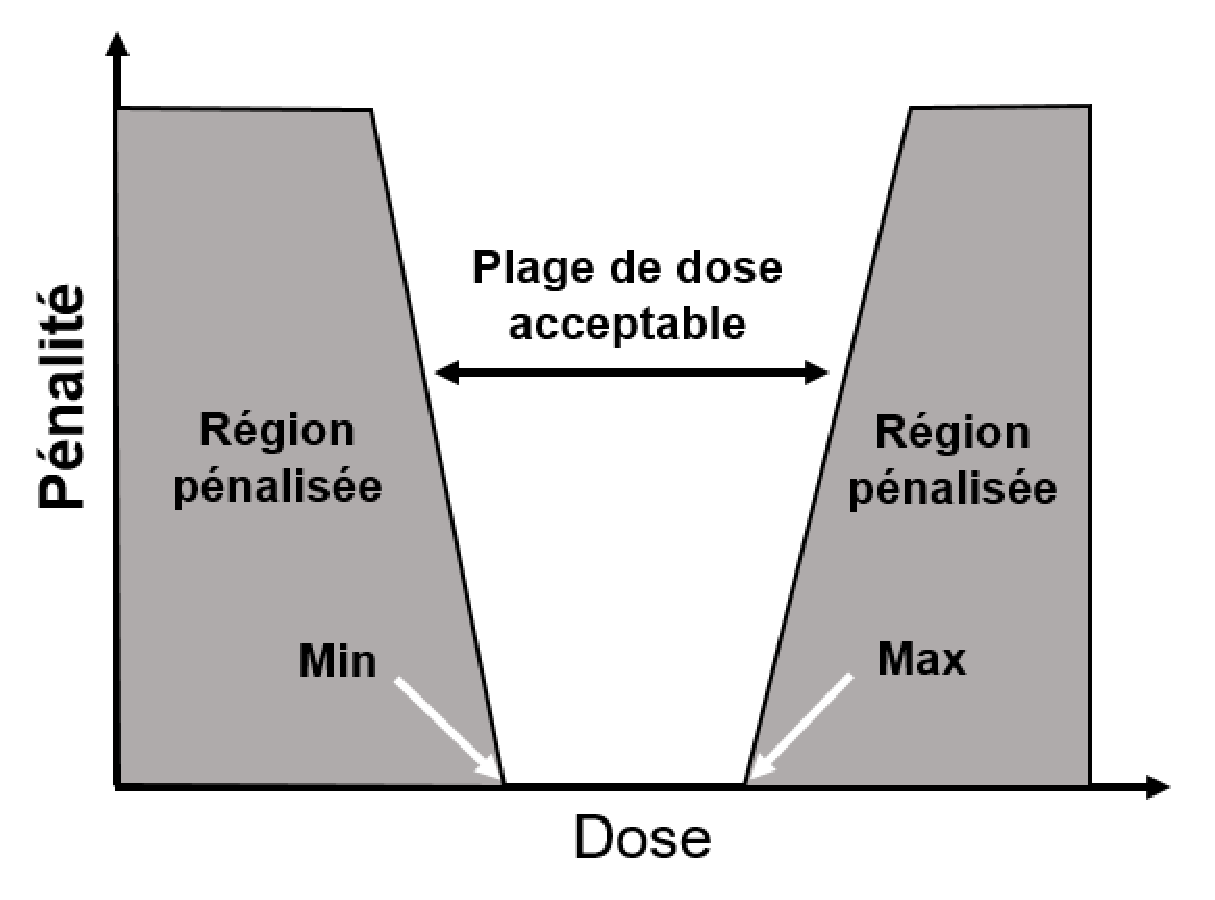
\includegraphics[width=7.5cm, height=6.0cm]{FigurePenalite}
\caption{\label{FigurePenalite} Illustration des différentes régions de dose acceptable et pénalisée.}
\end{figure}
%
D$_{min}$ et D$_{max}$ sont respectivement la valeur minimale et maximale délimitant la plage de dose acceptable. Pour la couverture du CTV par exemple, une dose dans la plage acceptable correspond à une pénalité nulle et à l’extérieure de celle-ci, à une pénalité qui augmente avec un taux égal à m$_{min}$ et m$_{max}$, respectivement pour toute dose D$_{i}$ < D$_{min}$ et D$_{i}$ > D$_{max}$. Le contrôle par le planificateur sur l’ajustement des pentes m$_{min}$ et m$_{max}$ lui permet donc de fixer les importances relatives entre les différents critères cliniques. Plus la pente est élevée, plus la pénalité est forte pour la dose se situant à l’extérieur de la plage acceptable. IPSA permet ainsi de définir deux types de contraintes, à savoir, la contrainte de dose à la surface et dans le volume. Particulièrement pour le CTV, une contrainte de dose à la surface va forcer la conformité de la dose dans son volume, et la contrainte de dose en volume permettra le contrôle de l’homogénéité. On définit une fonction de coût globale qui est la somme de toutes les pénalités W$_{i}$ de la dose en chaque point $i$  pour les contraintes de surface et/ou de volume pour chaque volume d’intérêt (CTV, urètre, vessie, rectum). Cette fonction décrit mathématiquement les objectifs cliniques et est utilisée pour l’évaluation de la distribution de dose; plus cette dernière est proche de la distribution idéale, moins élevée sera la fonction de coût (minimum global).\newline.
%
\item[] \textbf{HIPO} (Hybrid Inverse Planning and Optimization) \nomenclature{HIPO}{Hybrid Inverse Planning and 				Optimization}\newline
Il s’agit d’un algorithme d’optimisation hybride, développé en 2005 pour la planification des traitements en curiethérapie HDD \cite{Karabis}. Le caractère hybride tient du fait que l’algorithme utilise deux méthodes de calcul: (1) le recuit simulé qui est une méthode empirique (métaheuristique) pour optimiser la distribution des cathéters, et (2) une méthode déterministe basée sur le gradient (L-BFGS) \nomenclature{L-BFGS}{Limited-memory Broyden-Fletcher-Goldfarb-Shanno} pour l’optimisation de la distribution de dose. La construction de la fonction coût est basée sur les contraintes de dose en volume et celle-ci pénalise les valeurs de dose qui sont extérieures à la plage de dose acceptable pour chaque structure. Les bornes inférieure ($f_{inf}$) et supérieure ($f_{sup}$) de cette plage de dose sont définies par l’équation \eqref{eqn:FL} pour le CTV et l’équation \eqref{eqn:FH} pour le CTV, les OARs et les tissus normaux (NT), c'est-à-dire, les tissus situés à l'extérieur du CTV et pour lesquels aucun OAR n'est définit: 
%
\newcommand{\vect}[1]{\boldsymbol{#1}}
\begin{equation}\label{eqn:FL}
f_{inf}(\mathbf{x})=\frac{1}{n}\sum^{n}_{i=1}\Theta\left(D_{inf}-d_{i}(\mathbf{x})\right)\left[D_{inf}-d_{i}(\mathbf{x})\right]
\end{equation}
%
\begin{equation}\label{eqn:FH}
f_{sup}(\mathbf{x})=\frac{1}{n}\sum^{n}_{i=1}\Theta\left(d_{i}(\mathbf{x})-D_{sup}\right)\left[d_{i}(\mathbf{x})-D_{sup}\right]
\end{equation}
%
$n$ est le nombre de points distribués dans le CTV, NT et OARs. D$_{inf}$ et D$_{sup}$ sont respectivement la borne inférieure et supérieure de la plage de dose acceptable. $\mathbf{x}$ est un vecteur de variables indépendantes assujetties à l’optimisation (nombre de cathéters, dwell positions, dwell times, etc.), d$_{i}(\mathbf{x})$ la dose calculée au point $i$ du volume d’intérêt et $\Theta$ la fonction de Heaviside \cite{Pokharel} définit par l’équation \eqref{eqn:Transition}: 
%
\begin{equation}\label{eqn:Transition}
    \Theta (\beta) = \begin{cases}
              1              & \qquad si \quad \beta > 0 \\
              0,5            & \qquad si \quad \beta = 0 \\	
              0 			 & \qquad si \quad \beta < 0
           \end{cases}
\end{equation}
%
La fonction de coût global utilisée par l'algorithme HIPO est la somme pondérée de f$_{inf}$ et f$_{sup}$ définit pour chaque volume d'intérêt (CTV, volume boost, OARs), selon l'équatiom:
%
\begin{equation}\label{eqn:FGlobal}
f=w_{1}f^{CTV}_{inf}+w_{2}f^{CTV}_{sup}+w_{3}f^{NT}_{sup}+\sum^{OARs}_{j=1}w_{j+3}f^{jOAR}_{sup}
\end{equation}
%
Un des avantages de l’algorithme HIPO est sa capacité à bloquer les positions de certains cathéters en les retirant du processus d’optimisation et le contrôle des temps d’arrêt élevés \cite{EPoulin}.\newline
%
\item[] \textbf{DVHO} (Dose-Volume Histogram based Optimization) \nomenclature{DVHO}{Dose-Volume Histogram based 					Optimization}\newline
La méthode d’optimisation DVHO est une méthode qui repose sur les objectifs de dose ($f_{inf}, f_{sup}$) tels que définis dans les équations \eqref{eqn:FL} et \eqref{eqn:FH} pour chaque volume d’intérêt. La minimisation de la valeur de la fonction de coût se fait donc avec le même algorithme que HIPO, mais avec une approche de calcul différente. En effet, le planificateur définit les objectifs de dose directement sur les histogrammes dose-volume (DVH) \nomenclature{DVH}{Dose-Volume Histogram} et l’algorithme DVHO se charge de réduire de façon itérative, le volume recevant une dose inférieure à $f_{inf}$ et supérieures à $f_{sup}$ pour le CTV (réduction des points chauds et froids), et celui recevant une dose supérieure à $f_{sup}$  pour les OARs, ceci dans l’objectif de générer les DVHs proches des objectifs cliniques. Un complément descriptif de cet algorithme peut être trouvé dans l’ouvrage de Dimos Baltas \cite{Baltas}, ainsi que son évaluation comparativement à l’algorithme HIPO dans les travaux de Pokharel et al.\cite{Pokharel}.
\end{itemize}
% 
\subsection{Outils d'évaluation d'un plan}
La qualité d’un plan du point de vue de la radiobiologie est déterminée par deux indices, la probabilité de contrôle tumoral, TCP (Tumor Control Probability) \nomenclature{TCP}{Tumor Control Probability} \cite{Okunieff} et la probabilité de complication des tissus normaux, NTCP (Normal Tissue Complication Probability) \nomenclature{NTCP}{Normal Tissue Complication Probability} \cite{Lyman, Niemierko, Emami}. Cependant, la plupart des TPS ne permettent pas encore d’accéder en temps réel à ces indices au cours d’un processus de planification de traitement,  ces deux indices sont donc noyés dans l’évaluation de la dosimétrie physique. Du point de vue physique, l’évaluation de la qualité d’un plan en radiothérapie inclut les aspects relatifs à la couverture du CTV, l’homogénéité de la dose dans celui-ci et la dose délivrée aux OARs. L’évaluation peut se faire qualitativement et quantitativement. L’évaluation qualitative est faite par une visualisation des courbes d'isodoses sur chaque coupe CT, indépendamment de la modalité de traitement (détection des points chauds et froids). Particulièrement en curiethérapie, l’évaluation quantitative repose sur un ensemble d’indices tels que \cite{Kehwar, Prabhakar, Anbumani, Saw}:\newline
%
\begin{itemize}[leftmargin=0pt, label=\textbullet, font=\LARGE]
\item[] \textbf{Indice de couverture} (CI : Coverage Index) \nomenclature{CI}{Coverage Index}\newline
Fraction du volume cible (CTV)  qui reçoit une dose supérieure ou égale à la dose de référence D$_{ref}$.
%
\begin{equation}\label{eqn:CI}
CI=\frac{V_{D_{ref}}}{V_{CTV}}
\end{equation}
%
\item[] \textbf{Indice volumique externe} (EI:  External Volume Index) \nomenclature{EI}{External Volume Index}\newline
Volume des tissus normaux (NTV$_{D_{ref}}$) qui reçoit une dose supérieure ou égale à la dose de référence D$_{ref}$, normalisé au volume du CTV.
%
\begin{equation}\label{eqn:EI}
EI=\frac{NTV_{D_{ref}}}{V_{CTV}}
\end{equation}
%
\item[] \textbf{Indice relatif d’homogénéité} (DHI: Relative Dose Homogeneity Index) \nomenclature{DHI}{Relative Dose Homogeneity Index}\newline 
Volume du CTV qui reçoit une dose dans la plage 1,0 à 1,5 fois la dose de référence, normalisé au volume du CTV qui reçoit une dose supérieure ou égale à la dose de référence.
%
\begin{equation}\label{eqn:DHI}
DHI=\frac{V_{D_{ref}}-V_{1,5D_{ref}}}{V_{D_{ref}}}
\end{equation}
%
\item[] \textbf{Indice volumique de surdosage} (ODI: Overdose Volume Index) \nomenclature{ODI}{Overdose Volume Index}\newline
Rapport entre le volume cible qui reçoit une dose supérieure ou égale à deux fois la dose de référence, et le volume cible qui reçoit une dose supérieure ou égale à la dose de référence.
%
\begin{equation}\label{eqn:ODI}
ODI=\frac{V_{2D_{ref}}}{V_{D_{ref}}}
\end{equation}
%
\item[] \textbf{Pourcentage de non conformité} (DNR : Dose Non-uniformity Ratio) \nomenclature{DNR}{Dose Non-uniformity Ratio}\newline
Volume du CTV qui reçoit une dose supérieure ou égale 1,5 fois la dose de référence, normalisé au volume du CTV qui reçoit une dose supérieure ou égale à la dose de référence.
%
\begin{equation}\label{eqn:DNR}
DNR=\frac{V_{1,5D_{ref}}}{V_{D_{ref}}}
\end{equation}
%
\end{itemize}
Un implant idéal correspond à une situation où CI = 1, EI = 0, DHI = 1, ODI = 0 et DNR = 0. En plus de ces indices définis ci-dessus, la qualité des plans est également analysée à l’aide des DVHs (DVH cumulatif et/ou différentiel), le type le plus utilisé étant le DVH cumulatif (forme intégrale). Le DVH cumulatif est la représentation graphique de la distribution de dose à l’intérieur d’un certain volume (CTV, OARs). Pour construire un DVH cumulatif, on procède d’abord à la discrétisation de la dose en de petits intervalles [D$_{i}$, D$_{i+1}$] appelés classes de dose auxquelles correspond un volume V$_{clas}$. Chaque point de l’histogramme a pour coordonnée sur l’axe des abscisses, la valeur du centre de la classe $i$ et pour ordonnée, son volume ou le pourcentage du volume qui reçoit une dose supérieure ou égale à la valeur de la dose de cette classe. Le DVH cumulatif permet donc quantifier sur son graphe, le pourcentage du volume d’intérêt recevant au moins une dose donnée, ce qui rend possible l’analyse rapide sur la couverture du CTV et le degré par lequel les OARs sont épargnés. D’autre part, plusieurs études ont montré la corrélation des DVHs avec la toxicité \cite{Fiorino, Rodrigues, Taussky, Geinitz}.  Les différents indices décrits précédemment peuvent également être extraits des DVHs, c’est-à-dire, V$_{x}$: le volume recevant au moins un pourcentage $x$ de la dose de prescription et D$_{x}$: la dose reçue par un pourcentage $x$ du volume. En choisissant des classes de dose assez petites, un DVH cumulatif prend l’apparence la figure \ref{DVH}  ci-dessous.
%
\begin{figure}[!ht]
\centering
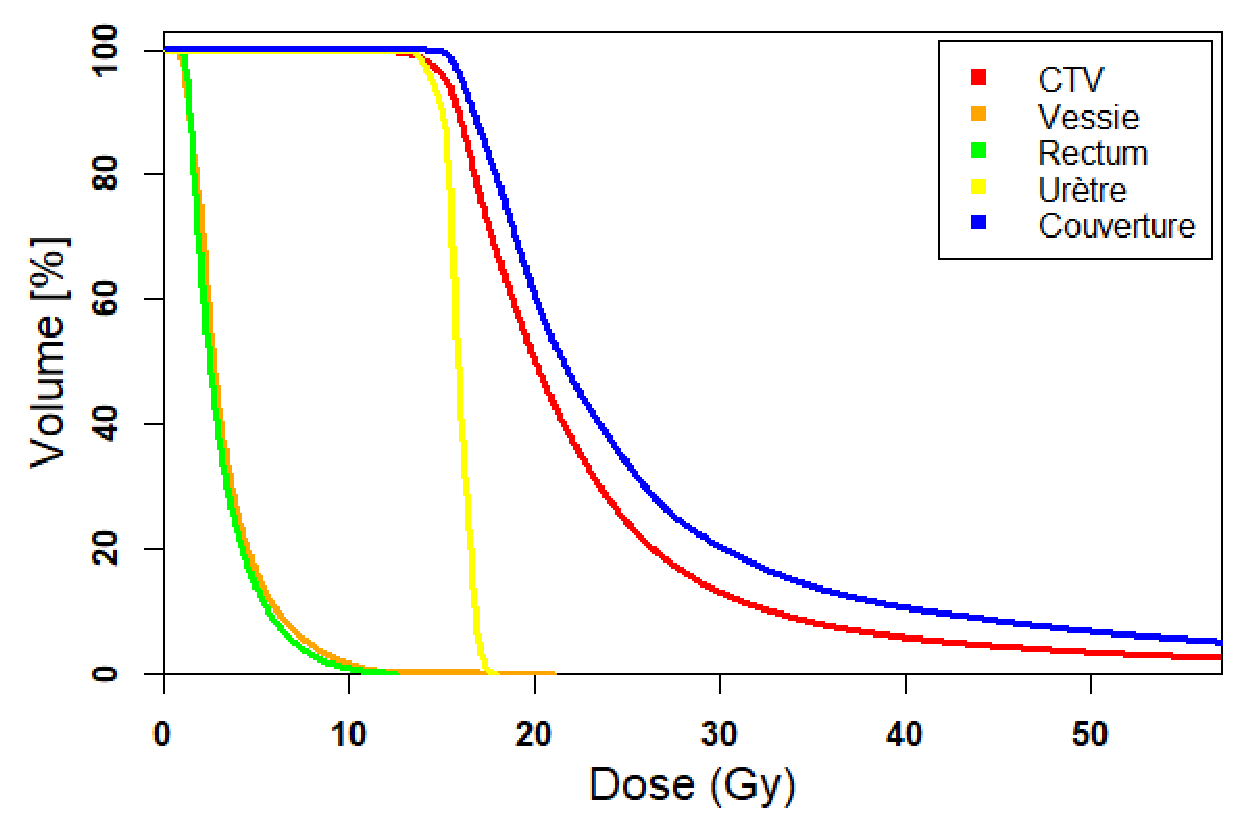
\includegraphics[width=9.0cm, height=6.5cm]{DVH.eps}
\caption{\label{DVH}Exemple d’un DVH cumulatif pour une prostate traitée en curiethérapie HDD en une séance de 15Gy, en complément à la radiothérapie externe (boost).}
\end{figure}
%
L’inconvénient majeur de cet outil est l’absence totale de l’information spatiale, c’est-à-dire, aucune localisation géométrique des volumes extraits des DVHs n’est possible, d’où la complémentarité de cet outil avec ceux décrits précédemment.
%
\newpage
\section{Description du projet de recherche}
Le présent projet porte sur la curiethérapie de la prostate HDD dont le développement a eu un regain d’intérêt dans les années 1980, après que Halm et al. \cite{Holm2002} aient démontré dans leurs travaux que la radiographie ultrason transrectal pouvait être utilisée pour guider la réalisation des implants prostatiques avec une meilleure précision. Cette approche est utilisée aujourd’hui par plusieurs centres de radiothérapie pour les traitements en curiethérapie HDD avec les projecteurs de sources équipés de sources d’Iridium-192 \cite{Stromberg, Mate, Borghede, Hoskin, Demanes, Blasko}. La réalisation des objectifs cliniques en termes de conformité de la dose au volume cible et limitation de la dose aux tissus et organes à risques (OARs) \nomenclature{OAR}{Organe à risque (Organs At Risk)} dépend d’une part, de la précision avec laquelle les cathéters sont implantés dans la glande, et d’autre part, de la méthode d’optimisation utilisée par le TPS. Les premières méthodes d’optimisation traditionnelles les plus utilisées étaient l’optimisation géométrique et l’optimisation par points de dose \cite{Ezzel, Thomadsen, Edmundson1, Edmundson2}. Un des points caractéristiques communs à ces deux méthodes est la nécessité d’une forte interaction entre le planificateur et le TPS, \nomenclature{TPS}{Système de planification de traitement (Treatment Planning Systems)} car ce dernier doit essayer plusieurs combinaisons de positions actives au sein de chaque cathéter, ainsi que les poids respectifs associés à chacune des positions, afin d’obtenir une distribution de dose satisfaisante, c’est-à-dire, qui respecte les objectifs cliniques. Cette dépendance, non seulement augmente la durée de la planification, mais conduit aussi à un plan final dont la qualité dépend du jugement et de l’expérience du planificateur. Le développement de la planification inverse avec l’algorithme IPSA \cite{ELessard, LessardP, Lessard2004} a permis l’automatisation de certaines tâches. Cette classe d’algorithme est caractérisée par la définition d’une fonction de coût qui reflète les objectifs cliniques et les contraintes de dose aux tissus sains (section \ref{sssec:optimis}). L’interaction entre le planificateur et le TPS se trouve ainsi réduite, car l’algorithme IPSA détermine automatiquement les positions à activer au sein de chaque cathéter (dwell positions), ainsi que le temps d’arrêt à chacune des positions (dwell time). Cependant, le processus d’optimisation demeure itératif et la qualité du plan reste dépendante du jugement du planificateur et de son expérience, puisque la solution optimale calculée par l’algorithme reste dépendante de la combinaison des pénalités que le planificateur a imposées à chaque objectif et/ou contrainte. Les outils d’évaluation d’un plan (isodose, DVH, etc.) \nomenclature{DVH}{Histogrammes doses-volumes (Dose Volume Histogram)} reposent essentiellement sur les recommandations de la couverture de dose dans le volume cible, et la limite de celle-ci aux OARs, recommandations contenues dans les publications de certains organismes internationaux tels que le RTOG 0924 \cite{ RTOG} \nomenclature{RTOG}{ Radiation Therapy Oncology Group}  ou de l’American Brachytherapy Society (ABS) \nomenclature{ABS}{American Brachytherapy Society}\cite{ABS}. Ces recommandations sont basées sur les études d’inférence statistiques, et donc, ne prennent pas en compte les variations des paramètres géométriques inter-patients qui ont un impact sur le compromis à réaliser, entre la couverture du volume cible et la minimisation de la dose aux OARs. De plus, il n’existe aucun outil objectif permettant au planificateur de juger de la qualité du compromis obtenu dans l’atteinte des objectifs cliniques. On pourrait donc penser de ce qui précède que, quelles que soient la méthode d’optimisation utilisée et l’expérience du planificateur, le plan de traitement obtenu suite à un tel processus de planification, bien qu’il soit conforme aux objectifs cliniques, n’est pas nécessairement le plus optimal qu’il serait possible d’obtenir. Les insuffisances décrites ci-dessus suggèrent la nécessité de développer de nouveaux outils d’aide à la planification, d’où l’intérêt de ce projet dont l’objectif est d’introduire un nouveau concept de contrôle qualité en curiethérapie de la prostate HDD, grâce à l’analyse de frontière stochastique (AFS) \nomenclature{AFS}{Analyse de Frontière Stochastique} qui est une méthode économétrique \cite{Dennis}. L’application de l’AFS dans ce contexte conduira à la construction des modèles d’aide à l’optimisation des plans, grâce aux paramètres géométriques inter-patients. Ces modèles auront également un pouvoir prédictif sur les paramètres dosimétriques d’intérêt qui guident le processus de planification. Plusieurs études réalisées en radiothérapie par modulation d’intensité (IMRT) \nomenclature{IMRT}{Radithérapie par modulation d’intensité (Intensity Modulated Radiation Therapy)} ont montré que de telles corrélations (dose-paramètres géométrique) étaient possibles et pouvaient conduire à l’amélioration de la qualité des plans de traitement en IMRT \cite{LachanceB, KevinLM, MargieAH, Marie-Chantal}. Les modèles développés constitueront également un outil objectif dans l’évaluation de la qualité du compromis obtenu à la fin d’un processus de planification (couverture du volume cible vs minimisation de la dose aux OARs).
%
\section{Organisation du mémoire}
%\addcontentsline{toc}{section}{Organisation du mémoire}
Le présent travail est organisé en quatre parties. Après une introduction (chapitre 1) qui présente brièvement l'origine de la radiothérapie, et particulièrement la curiethérapie, les concepts d'assurance et contrôle qualité, la présentation du cancer de la prostate (incidence, mortalité, diagnostic et aspects dosimétriques), et la description des objectifs du présent projet, suivra le chapitre 2 consacré à la présentation du formalisme de l’analyse de frontière stochastique et son exploitation dans le cadre de ce projet pour l’optimisation des plans en curiethérapie de la prostate HDD. Un article résumant les résultats principaux de ce travail pour soumission au Brachytherapy Journal fait partie du chapitre 3, et une conclusion ainsi que des développements futurs du projet pour ces aspects cliques clôturent ce travail dans sa quatrième partie.
%